\chapter{Introducción}
\graphicspath{{figs/cap1/}}
\label{cap1}



En el estudio de la Mecánica de los Fluidos, son de importancia los problemas de transferencia de calor de flujos multifásicos con cambios de fase. Una de las áreas más relevantes en que se tratan estos problemas es la generación de energía eléctrica, ya sea por medio de fisión o fusión nuclear, la combustión de combustibles fósiles, fuentes de energía geotérmica entre otros \cite{incropera2007fundamentals}. Actualmente se estan investigando formas de eficientizar la producción de energía debido a que se espera un incremento de la demanda por la población \cite{schiffer2018world}.

% debido a que el Consejo Mundial de Energía (\textit{World Energy Council} o WEC) prevé que se debe realizar un aumento en la generación de energía\cite{schiffer2018world}, para satisfacer la creciente demanda eléctrica de la población. Por ello es que se investigan y desarrollan nuevos métodos para generar energía de una forma más eficiente. Entre las líneas de investigación que existen se encuentra la mejora de instalaciones existentes y para ello es necesario centrar los estudios de la física básica.
Una de las ramas de investigación es en la industria nuclear, en donde se pretende mejorar la eficiencia en la remoción del calor de las barras del elemento combustible hacia el fluido del circuito de refrigeración primario. En particular, resulta de interés evaluar dicha transferencia de calor mediante procesos de ebullición en el fluido que entra en contacto con los elementos combustibles. Sin embargo, la realización de experimentos resulta costosa debido a los recaudos de seguridad y equipos necesarios. Estas limitaciones intrínsecas motivan el desarrollo de modelos numéricos capaces de predecir adecuadamente los fenómenos involucrados \cite{zhang2011numerical}. 


%En la industria nuclear una de los problemas más complejos a resolver, es la transferencia de calor entre el fluido que circula en el circuito primario de refrigeración con las barras de elemento combustible, debido a que se produce el fenómeno de ebullición. Es de interés el estudio de dicho problema porque según la eficiencia con que se realice la remoción del calor queda determinada la potencia de trabajo del reactor nuclear.

% Uno de los más relevantes por su importancia en la aplicación industrial y que contínuamente está en investigación debido a su complejidad; es la interacción entre el fluido de un reactor nuclear con sus barras de elemento combustible.

%El punto crítico de calor (\textit{Critical Heat Flux} o CHF ) es aquél dónde la curva de Nukiyama de un material aumenta en varios órdenes de magnitud se temperatura si se incremente infinitesimalmente su potencia. Conocer el CHF de un reactor nuclear determina el punto de operación del mismo; debido a que el ente regulatorio nuclear que avala el funcionamiento de un reactor, determina la potencia de operación del mismo en base a la alcanzada en el CHF.
%
%Nukiyama estudió, en la curva que lleva su nombre, cómo es la variación de la temperatura según la potencia que se le esté aplicandoa un material inmerso en un fluido y describió con detalle las diferentes etapas del proceso de ebullición. Actualmente la única forma de validar el CHF de las barras de elemento combustible de un reactor es mediante ensayos experimentales, los cuáles insumen mucho tiempo de espera (años) para realizar su prueba, porque son escasos los lugares que cuentan con la tecnología para brindar el servicio, además de ser costosos. 
%
%Es de importancia contar con un código numérico que se encuentre validado, reproduzca la fenomenología de forma efectiva, sea fácil de utilizar cambiando la geometría y/o parámetros del fluido a utilizar. Los costos de fabricación disminuirían considerablemente al no ser necesaria una gran iteración de prototipos (en el problema mencionado).

Actualmente la dificultad para reproducir numéricamente los tipos de problemas mencionados es que debido a las escalas de fluido involucradas (\textit{mesoscópicas}), con las técnicas numéricas convencionales de Mecánica de Fluidos Computacional (\textit{Computational Fluid Mechanichs} o CFD) resulta difícil obtener resultados en un tiempo razonable y que también tengan en cuenta todos las interacciones físicas que ocurren \cite{guo2013lattice}. En parte es debido a que los métodos tradicionales resuelven ecuaciones diferenciales mediante técnicas de discretización que involucran la resolución numérica de grandes sistemas de ecuaciones, donde el tiempo de cálculo típicamente varía cuadráticamente con el número de elementos de malla utilizada para discretizar el problema físico.

Uno de los métodos numéricos que se están desarrollando para que el costo computacional sea cada vez menor es el método de lattice Boltzmann (\textit{lattice Boltzmann \\
Method} o LBM). Estos métodos resuelven las ecuaciones diferenciales por medio de una ecuación lineal más sencilla, lo cuál reduce drásticamente el tiempo de cálculo, y las variables que se obtienen cumplen con la ecuación de interés. Debido a que están basados en realizar operaciones elementales en los elementos de la malla discretizada y a su vez no dependen del total de nodos de la misma, se convierten en algoritmos altamente paralelizables.

Por lo mencionado anteriormente, el estudio de la transferencia de calor en flujos multifásicos con cambio de fase es difícil de modelar numéricamente y los métodos existentes son costosos computacionalmente. Esto implica que resulta necesario desarrollar e investigar nuevas técnicas numéricas junto con sus implementaciones, de modo que  sea posible resolver la fenomenología de interés con precisión y en tiempo razonable.

%\section{Descripción de las escalas de los fluidos}
%
%Los fluidos como el aire y el agua son conocidos en nuestra vida diaria. Físicamente los fluidos están compuestos de un gran conjunto de átomos o moléculas que chocan unas con otras moviéndose  aleatoriamente. Usualmente las interacciones de las moléculas de un fluido son más débiles que las de un sólido, por ello mediante la aplicación de un pequeño esfuerzo al fluido, éste puede ser deformado de manera continua.
%
%
%Usualmente la dinámica microscópica de las moléculas del fluido son muy complicadas y demuestran una fuerte inhomogeneidad y fluctuaciones.
%Por otro lado la dinámica macroscópica del fluido, el cual es el resultado medio del movimiento de las moléculas en un medio homogéneo y continuo.
%Mediante modelos matemáticos puede explicarse la dinámica de los fluidos , según el fluido observado y su fuerte dependencia del tamaño de su escala.
%
%La mecánica de los fluidos se puede describir en tres niveles: macroscópica, mesoscópica y microscópica.
%Generalmente el movimiento de un fluido puede ser descripto por tres tipos de modelos matemáticos acuerdo a lo que se observan en las distintas escalas, por ejemplo microscópico en modelos de escala molecular, teorías cinéticas en la escala mesoscópica y modelos continuos para escalas macroscópicas.
%
%
%Los modelos matemáticos de los flujos de fluidos son :
%
%\begin{itemize}
%	\item ecuación de Newton para una cantidad elevada de moléculas (escala microscópica)
%	\item ecuación de Boltzman para la función de distribución simple (escala mesoscópica)
%	\item ecuaciónes de aproximación de la mecánica del contínuo, como ser la ecuación de Navier-Stokes para macro-variaciones de flujos (escala macroscópica).
%\end{itemize}
%
%que resultan extremadamente difíciles de resolver analíticamente de no ser imposibles.
%
% La precisión de los modelos numéricos sin embargo han provisto de manera satisfactoria soluciones aproximadas de dichas ecuaciones.
%Particularmente con la rapidez del desarrollo del software y hardware computacional y la tecnología, las simulaciones numéricas han comenzado a ser una importante metodología para la dinámica de fluidos.
%
%Una de las vertientes de  investigación y aplicación más popular de simulación de fluidos es la técnica Mecánica de Fluidos Computacional (\textit{Computational Fluid Dynamics} o CFD) , el cual está diseñado para resolver ecuaciones hidrodinámicas basadas en supociones de continuidad. Siendo sus técnicas más difundidas la de elementos finitos, volúmenes finitos entre otras.
%En CFD el dominio del flujo está compuesto según la técnica \textit{meshless} utilizada, como  diferencia finitas; los cuales resultan en un sistema algebraico de sistemas de ecuaciones para las variables discretas del fluido asociadas a la malla computacional. 
%Computacionalmente son llevados a cabo para encontrar una solución aproximada resolviendo el problema algebraico de sistemas de ecuaciones usando un algoritmo secuencial o paralelo.
% 
%La Simulación de Dinámica Molecular (\textit{Molecular Dynamic Simulation} o MDS) es una técnica en la cual el movimiento individual de átomos o moléculas del fluido son registrados para resolver las ecuaciones de Newton.
%La principal ventaja de MDS es el aspecto macroscópico del fluido puede ser directamente conectado con el comportamiento molecular, en donde la estructura molecular y las interacciones microscópicas pueden ser descriptas de una manera directa.
%
%El método de lattice Boltzmann ( \textit{lattice Boltzman Method} o LBM) es una aproximación del nivel mesoscópica. LBM estudia la micro-dinámica de partículas ficticias utilizando modelos cinéticos simplificados, lo cual provee un camino alternativo de simular la mecánica de fluidos. La naturaleza de la cinética brinda distintas características de LBM tales que es claro el panorama de los procesos de advección y colisión de partículas de fluidos simuladas. La estructura del algoritmo es simple y de fácil implementación en las condiciones de contorno, además presenta un paralelismo natural. Todos éstos interesantes atributos hacen que LBM sea una potente herramienta numérica para la simulación de sistemas de fluidos envueltos en problemas físicos complejos\cite{guo2013lattice}. 


\section{Descripción general de LBM}

Tradicionalmente los problemas de mecánica de fluidos resueltos mediante la suposición del continuo son llevados a cabo mediante  ecuaciones como las de Navier-Stokes. Obtener la solución numérica de dichas ecuaciones implica resolver sistemas  algebraicos de ecuaciones, cuya cantidad está sujeta a la forma de realizar la discretización del espacio físico y según la cantidad de elementos de la malla. La resolución de este tipo de ecuaciones presenta la característica de que el tiempo de cálculo involucrado en su resolución depende típicamente de forma cuadŕatica con la cantidad de elementos discretizados \cite{kelley1995iterative}.

El LBM resuelve de manera indirecta las ecuaciones diferenciales, a través de la discretización de una ecuación de Boltzmann, lineal y de resolución numérica más sencilla. En particular, dichas ecuaciones representan el transporte de funciones de distribución, cuyos momentos en el espacio de fases pueden asociarse con propiedades macroscópicas del fluido, como densidad, velocidad o temperatura.

La discretización espacial que se suele utilizar es mediante un mallado regular \cite{guo2013lattice}, y  cada nodo de la malla tiene asignado un espacio de velocidades. Los modelos de grilla suelen denotarse como $DdQq$, donde \textit{d} son las dimensiones y \textit{q} la cantidad de componentes que se discretiza el espacio de velocidades. La figura \ref{fig:D1Q3_D2Q9} muestra cómo son los conjuntos de velocidades para los modelos D1Q3 y D1Q9.

El espacio de velocidades indica cómo es la propagación de las propiedades que poseen los nodos de la grilla. La velocidad de grilla del nodo i-ésimo se denota $\mathbf{e}_{i}$ y posee \textit{q} componentes. Para el modelo D2Q9 la figura \ref{fig:D1Q3_D2Q9} muestra un esquema de las velocidades de grilla del nodo i - ésimo y la Ec. (\ref{eq:velgrilla}) el valor adoptado. 

\begin{figure}[h!]
	\centering
	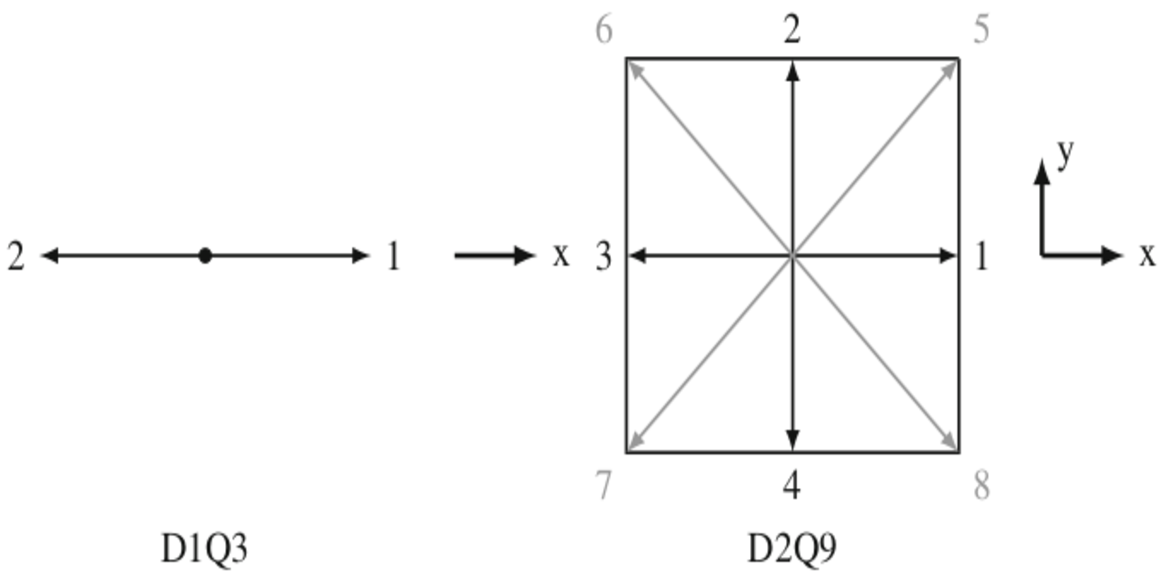
\includegraphics[width=.8\textwidth]{figs/cap1/D1Q3_D2Q9}
	\caption{Conjunto de velocidades de los modelos D1Q3 y D2Q9. \cite{kruger2017lattice}}
	\label{fig:D1Q3_D2Q9}	
\end{figure}


\begin{equation}
{\mathbf{e}_{i}} =  
\left( \begin{array}{c} 
e_{0} \\ e_{1}\\ e_{2}\\ e_{3}\\ e_{4}\\ e_{5}\\
e_{6}\\ e_{7}\\ e_{8}\\
\end{array}
\right) =
\left( \begin{array}{c} 
( 0, 0, 0) \\ ( 1, 0, 0) \\ ( 0, 1, 0) \\(-1, 0, 0) \\ ( 0,-1, 0) \\ ( 1, 1, 0) \\
(-1, 1, 0) \\ (-1,-1, 0) \\ ( 1,-1, 0)\\ 
\end{array}
\right) 
\label{eq:velgrilla}
\end{equation}

Para la resolución de los problems de transferencia de calor con flujos multifásicos y cambio de fase que se propuso estudiar, es necesario contar con un LBM adecuado. En particular, existen cuatro (4) categorías generales para clasificar los modelos multifásicos: color gradient, free energy, phase field y pseudopotential.

En este trabajo se utilizará la familia pseudopotencial, la cual está basada en proponer un potencial de interacción entre las partículas del fluido. Dicho potencial se utiliza para calcular la fuerza de interacción entre las partículas del fluido y está dado según una Ecuación de estado (\textit{Equation of state o EOS}). 

A continuación se datallará un ejemplo sencillo de un modelo D2Q9. La Figura (\ref{fig:grilla_D2Q9}) muestra un esquema de las direcciones de las velocidades de grilla del nodo i-ésimo. En la misma figura se esquematiza cómo  es el proceso de colisión y advección (\textit{streaming}) que se realiza para actualizar los estados de los nodos cuando transcurre un paso de tiempo de la discretización temporal del problema. 


\begin{figure}[h!]
	\centering
	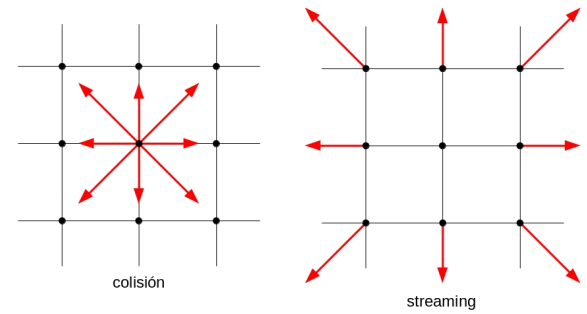
\includegraphics[width=8cm]{grilla_stre_colli_intro.png}
	\caption{Colisión y streaming de un modelo D2Q9 de LBM.}
	\label{fig:grilla_D2Q9}
\end{figure}

\newpage


\begin{align}
	\mathbf{f}_{\alpha} (\mathbf{x} + \mathbf{e}_{\alpha} \mathbf{\delta}_{t}, t + \mathbf{\delta}_{t})  = \mathbf{f}_{\alpha} (\mathbf{x}, t) - \frac{1}{\tau} (\mathbf{f}_{\alpha} - {\mathbf{f}_{\alpha}}^{eq})
	\label{eq:field_intro} 
\end{align}

El término derecho de la Ec. (\ref{eq:field_intro}) se conoce como \textit{colisión} y el izquierdo como \textit{streaming}; $\alpha$ corresponde al  $\alpha$-ésimo componente  ($\alpha = 0, 1, ... ,8$), $f^{eq}$ es la función de distribución en estado de equilibrio, $\tau$ es un parámetro de relajación del modelo que determina propiedades macroscópicas como la viscosidad.

Por medio de la \textit{colisión} y luego del \textit{streaming} se obtienen los parámetros macroscópicos el problema. Para éste caso sencillo se obtiene $\rho$ y $\mathbf{u}$ de las Ec. (\ref{eq: rho.1}) y (\ref{eq: u.1}) respectivamente.
\begin{align}
	\rho = \sum_{\alpha} \mathbf{f}_{\alpha}
	\label{eq: rho.1}
\end{align}
\begin{align}
	\rho \mathbf{u}= \sum_{\alpha} \mathbf{e}_{\alpha} \mathbf{f}_{\alpha}
	\label{eq: u.1}
\end{align}

\begin{figure}[H]
	\centering
	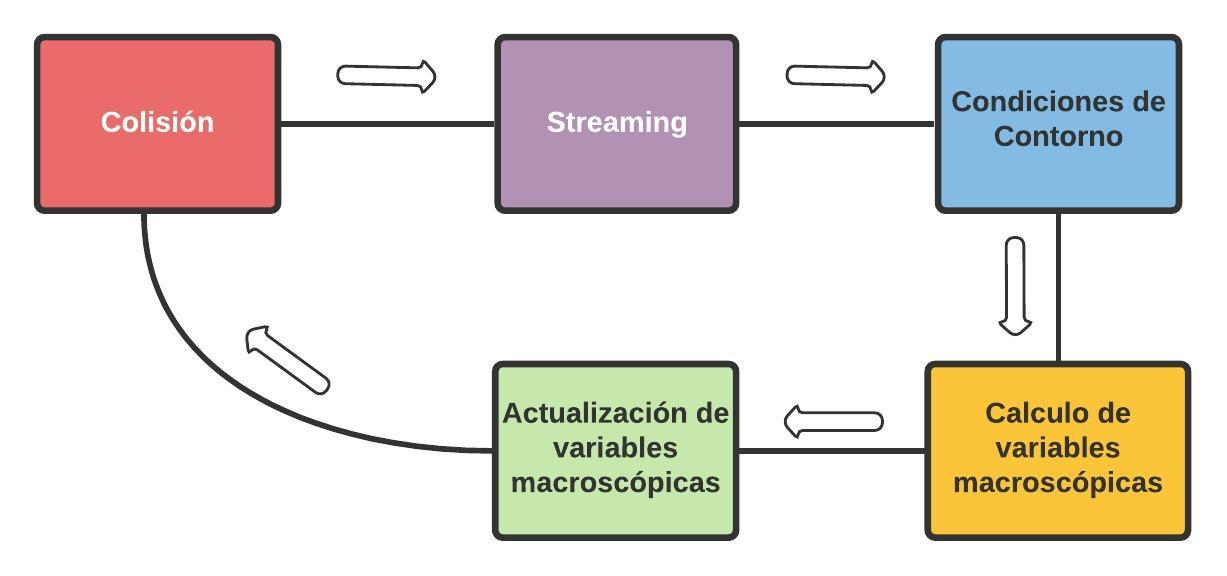
\includegraphics[width=14cm]{figs/cap1/esquema_LBM}
	\caption{Esquema de resolución de un método numérico de LB.}
	\label{fig:esquema_lbm}
\end{figure}

La Figura (\ref{fig:esquema_lbm}) muestra el esquema de resolución para el LBM descripto, donde primero se realiza la colisión de los nodos para luego mediante el \textit{streaming} actualizar en todos los nodos el valor de \textit{f}. A partir de ahí se deben aplicar las condiciones de contorno que pueda tener el problema y calcular las variables macroscópicas del sistema. Una vez realizada la actualización de las variables macroscópicas se recupera la solución de la ecuación diferencial de interés. El proceso descripto debe aplicarse en cada paso de tiempo.

Debido a que cada nodo de la grilla debe realizar la misma operación de colisión de manera independiente del resto, el modelo es altamente paralelizable. Además, las operaciones matemáticas que deben ejecutarse en el operador de colisión son sencillas, no implicando un gran costo computacional.

Por lo que se describió anteriormente, el LBM permite resolver indirectamente una ecuación, o EDP no lineal a partir de una ecuación lineal más sencilla y es paralelizable. Por lo tanto, esto motiva el desarrollo de códigos numéricos en unidades de procesamiento gráfico (\textit{Graphics Processing Unit} o GPU).
\newpage
\section{Descripción GPU}

Una Unidad de Procesamiento Gráfico (\textit{Graphics Processing Unit} o GPU) es un  circuito electrónico diseñado para realizar operaciones con punto flotante para renderizar píxeles en una pantalla. Están optimizadas para actuar en paralelo de forma simultánea instrucciones simples.

La GPU trabaja en conjunto con una Unidad Central de Procesamiento (\textit{Central Processing Unit} o CPU), debido a ello no presenta circuitos de control en su arquitectura. Dicho espacio que se encuentra ocupado en las CPU por el circuito de control las GPU lo disponen para incrementar el espacio en su chip de Unidades Aritmético Lógicas (\textit{Arithmetic Logic Unit} o ALU).

El esquema de la Figura (\ref{fig:cpu_gpu_transis}) muestra cualitativamente la cantidad de transistores dedicados a diferentes tareas en la CPU comparado con la GPU.

\begin{figure}[h!]
	\centering
	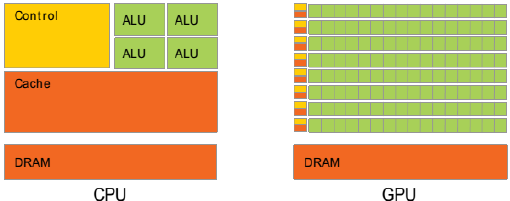
\includegraphics[width=10cm]{cpu_gpu.png}
	\caption{Comparación cualitatica del uso de transistores entre CPU y GPU \cite{rinaldi2011modelos}.}
	\label{fig:cpu_gpu_transis}
\end{figure}

Las GPUs estan acondicionadas para llevar a cabo los cálculos que presentan los métodos numéricos de LB. Los LBM consisten en que a cada uno de los nodos de la grilla discretizada se le realicen operaciones elementales como los de la Ec. (\ref{eq:field_intro}). Las GPU se encuentran optimizadas para ejecutar cálculos sobre los píxeles de un monitor, los cuales pueden considerarse como una grilla de nodos. A través de la paralelización la performance de las GPUs es alta, siendo capaces de procesar múltiples vértices y píxeles simultáneamente. Las simulaciones numéricas se producen en un menor tiempo en las GPU que sobre las CPU debido al alto paralelismo alcanzado por la GPU \cite{rinaldi2011modelos}.


El lenguaje de programación que se utilizó para trabajar con placas gráficas es \textsc{Cuda C} y fue desarrollado mediante la empresea NVIDIA. Se basa en el lenguaje de programación \textsc{C} con ciertas modificaciones para que los procesos sean en paralelo. Dichos procesos se especifican para que puedan ser lanzados en un número de \textit{blocks} y \textit{threads} de ejecución.

\newpage

\section{Descripción y alcance del proyecto integrador}

En el presente trabajo se implementó un código numérico para resolver problemas de transferencia de calor en flujos multifásicos con cambio de fase usando GPU de la forma más robusta posible. El LBM utilizado es el desarrollado por Fogliatto et al \cite{fogliatto2018modelado}, \cite{fogliatto2019simulation}, \cite{fogliatto2019transferencia}, y resuelve numéricamente problemas con discretización espacial de dominio regular en una grilla de tipo D2Q9.

El código numérico fue desarrollado usando el software \textsc{Git} debido a que permite llevar a cabo un control de versiones de manera robusta y sencilla. El repositorio donde se encuentra alojado el proyecto está en la página web de \textsc{Git Hub} y puede ser desacargado de \url{https://github.com/efogliatto/LBCUDA_Test/}. 

El código realizado utilizó el software \textsc{CMake} para preparar la compilación del código desarrollado, el cual permite desarrollar proyectos que posean una gran cantidad de directorios de forma simple. El código se encuentra implementado en tres lenguajes de programación, siendo ellos \textsc{C}, \textsc{Cuda C} y \textsc{Python}. Las bibliotecas generadas son del tipo \textit{shared} y \textit{static} para el caso de \textsc{C} y \textsc{Cuda C} respectivamente. Adicionalmente los \textit{kernels} de \textit{Cuda C} se compilaron en el formato tipo \textsc{ptx} para ser utilizadas mediante \textsc{Python} por medio del módulo \textsc{PyCuda}.

La validación del código fue realizado en dos PC diferentes, la primera contaba con una CPU Intel Core i7-3770 con una GPU NVIDIA GeForce GTX 760 y la segunda con una CPU Intel Core i7-4770 con una GPU NVIDIA GeForce GTX 970. A su vez la validación se concretó en variables de simple precisión y doble precisión, a través de la resolución de diferentes problemas numéricos (detallados en el Cap. (\ref{cap4})):

\begin{itemize}
	\item \textit{construcción de Maxwell}
	\item \textit{estratificación de un fluido Van der Waals (VdW) con temperatura no uniforme}
	\item \textit{generación de burbujas sobre una superficie horizontal calefaccionada}
\end{itemize} 

Se realizó una comparación de tiempos de cálculo entre los códigos de \textsc{C} y en \textsc{CUDA C} para ambas precisiones. Luego se realizó una comparación entre los tiempos de cálculo de simple precisión y doble precisión en el código de \textsc{Cuda C}.

Además, se usaron \textit{kernels} compilados en formato \textsc{ptx} de \textsc{Cuda C} dentro de \textit{scripts} de \textsc{Python} usando \textsc{PyCuda}, y se realizó una comparación de tiempos entre \textsc{Cuda C} y \textsc{Python}.


%%% Local Variables: 
%%% mode: latex
%%% TeX-master: "template"
%%% End: 
